\newpage
\begin{theorem}
    (Второй критерий квадрируемости)\\
    Фигура $A$ квадрируема $\Leftrightarrow \mu(\partial A)=0$.
\end{theorem}
\begin{proof}\tab
    \begin{itemize}
        \item[$(\Rightarrow):$] $A$ - квадрируема $\Rightarrow$ по первому критерию квадрируемости:
        \[\forall \epsilon>0\ \exists\ P_{\epsilon},\ Q_{\epsilon}: \mu(P_{\epsilon})-\mu(Q_{\epsilon}) <\epsilon\]
        $\partial A\subset P\setminus Q,\ Q$ - внутренние точки $A,\ \R^2\setminus P$ - внешние точки $A$.\\
        В частности,\ $\partial A\subset P_{\epsilon}\setminus Q_{\epsilon} \Rightarrow \mu^*(\partial A)<\epsilon \Rightarrow \mu(\partial A)=0$.
        \item[$(\Leftarrow):$] 
        $\mu(\partial A)=0 \Rightarrow \forall \epsilon>0\ \exists\ P_{\epsilon}\supset \partial A,\ \mu(P_{\epsilon})<\epsilon \Rightarrow \exists\ h>0,\\
        \partial A\subset \cup (\text{кв. сетка с шагом h})=A_2: \mu(A_2)<72\epsilon$ (по лемме ниже).\\
        $A_1=\cup(\text{квадраты сетки, целиком состоящие из внутренних точек A})\\
        \Rightarrow A\subset A_1\cup A_2 \Rightarrow A_1\cup A_2=P,\ A_1=Q,\ \mu(P)-\mu(Q)=\mu(A_2)<72\epsilon$
    \end{itemize}
\end{proof} 
\begin{lemma}
    Пусть $P$ - многоугольная фигура, $B\subset P$ и $\mu(P)<\epsilon \Rightarrow\ \exists\ h>0$ такое, что $B\subset M,\ \mu(M)<72\epsilon$, где $M$ - квадратная сетка со сторонами квадратов параллельными осям координат и шагом $h$.
\end{lemma}   
\begin{proof} Пусть $\mu(P)<\epsilon$
    \begin{enumerate}
        \item $P$ - многоугольная фигура $\Rightarrow P$ - это объединение треугольников\\
        $\Rightarrow P$ можно представить в виде объединения прямоугольных треугольников. Достроим прямоугольные треугольники до прямоугольников, их объединение обозначим $M_1$. Тогда $P\subset M_1$ и $\mu(M_1)<2\epsilon.$
        \item Теперь накроем $M_1$ объединением квадратов $M_2$. Будем накрывать прямоугольник квадратами со стороной, равной меньшей из сторон прямоугольника, начиная от одной из меньших сторон, пока не заложим весь прямоугольник. Тогда либо прямоугольник накрылся, либо последний квадрат вылез за границу, а так как площадь прямоугольника не меньше квадрата с его меньшей стороной, то площадь увеличилась не более чем вдвое (на самом деле строго меньше, но нам это не особо нужно). Итак, $M_1\subset M_2$ и $\mu(M_2)< 4\epsilon$.
        \begin{center}
            \begin{tikzpicture}
                \draw[->] (-0.3, 0) -- (6, 0) node[right] {x};
                \draw[->] (0, -0.3) -- (0, 4) node[above] {y};        
                \draw[thick] (1, 1) rectangle (3.5, 3);
                \draw[dashed] (3, 1) rectangle (5, 3);
            \end{tikzpicture}
        \end{center}
        \item Теперь накроем $M_2$ объединением квадратов $M_3$ таким, что стороны квадратов из $M_3$ параллельны осям координат. Для этого впишем каждый квадрат в квадрат со сторонами, параллельными осям (проведем параллели через вершины квадрата), тогда квадрат дополняется до нужного нам четырьмя треугольниками, причём квадрат разбивается на 4 равных треугольника, дополняющих изначальные до прямоугольников, плюс квадратный кусочек в центре, которого не будет только в случае поворота на 45 градусов - опять же площадь увеличится не больше чем вдвое. Значит, $M_2 \subset M_3$ и $\mu(M_3)< 8\epsilon$.
        \[
        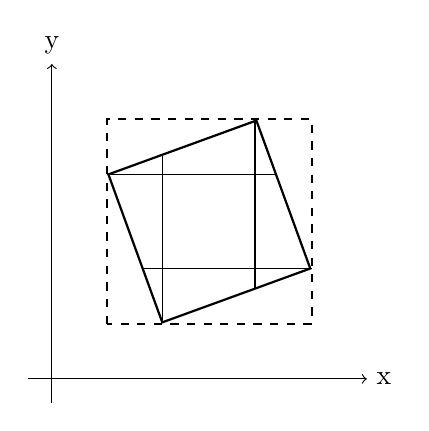
\begin{tikzpicture}
            \draw[->] (-0.3, 0) -- (4, 0) node[right] {x};
            \draw[->] (0, -0.3) -- (0, 4) node[above] {y};
            \draw[thick, rotate around={20:(2,2)}] (1, 1) rectangle (3, 3);
            \draw[thick, dashed] (0.7, 0.7) rectangle (3.3, 3.3);
            \draw[-] (0.7, 2.6) -- (2.85, 2.6);
            \draw[-] (1.15, 1.4) -- (3.3, 1.4);
            \draw[-] (1.4, 0.75) -- (1.4, 2.85);
            \draw[-] (2.58, 1.15) -- (2.58, 3.3);
        \end{tikzpicture}
        \tab[80pt]
        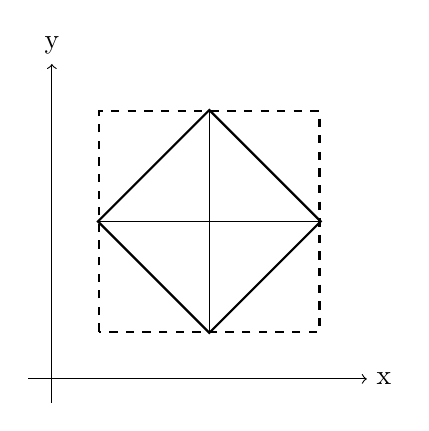
\begin{tikzpicture}
            \draw[->] (-0.3, 0) -- (4, 0) node[right] {x};
            \draw[->] (0, -0.3) -- (0, 4) node[above] {y};
            \draw[thick, rotate around={45:(2,2)}] (1, 1) rectangle (3, 3);
            \draw[thick, dashed] (0.6, 0.6) rectangle (3.4, 3.4);
            \draw[-] (2, 0.6) -- (2, 3.4);
            \draw[-] (0.6, 2) -- (3.4, 2);
        \end{tikzpicture}
        \]
        \item Теперь возьмем $h$, равное стороне наименьшего квадрата, и построим квадратную сетку $M$ с шагом $h$. Рассмотрим квдарат $L$, возможны два случая:
        \begin{itemize}
            \item[(i)] Если внутри квадрата $L$ ни один из квадратов сетки не лежит целиком $\Rightarrow L$ лежит внутри квадрата $2\times 2$, составленного из квадратов сетки. Поскольку площадь $L$ не не меньше площади квадрата сетки, то площадь увелисится не более чем вчетверо.
            \item[(ii)] Если существуют квадраты сетки, лежащие внутри $L$, то их объединение образует большой квадрат, лежащий внутри $L$, а значит весь $L$ покрывается девятью копиями этого квадрата.
        \end{itemize}
        \[
        \begin{tikzpicture}
            \draw[->] (-0.3, 0) -- (4, 0) node[right] {x};
            \draw[->] (0, -0.3) -- (0, 4) node[above] {y};
            \draw[thick] (1.5, 1.5) rectangle (2.5, 2.5);
            \draw[thick, dashed] (1.1, 1.1) rectangle (1.9, 1.9);
            \draw[thick, dashed] (1.1, 1.9) rectangle (1.9, 2.7);
            \draw[thick, dashed] (1.9, 1.1) rectangle (2.7, 1.9);
            \draw[thick, dashed] (1.9, 1.9) rectangle (2.7, 2.7);
        \end{tikzpicture}
        \tab[80pt]
        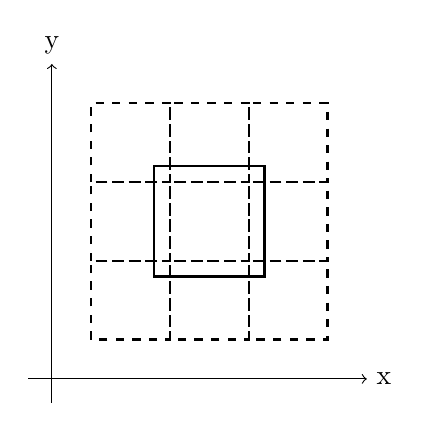
\begin{tikzpicture}
            \draw[->] (-0.3, 0) -- (4, 0) node[right] {x};
            \draw[->] (0, -0.3) -- (0, 4) node[above] {y};
            \draw[thick, dashed] (1.5, 1.5) rectangle (2.5, 2.5);
            \draw[thick] (1.3, 1.3) rectangle (2.7, 2.7);
            \draw[thick, dashed] (0.5, 0.5) rectangle (1.5, 1.5);
            \draw[thick, dashed] (0.5, 1.5) rectangle (1.5, 2.5);
            \draw[thick, dashed] (0.5, 2.5) rectangle (1.5, 3.5);
            \draw[thick, dashed] (1.5, 2.5) rectangle (2.5, 3.5);
            \draw[thick, dashed] (2.5, 2.5) rectangle (3.5, 3.5);
            \draw[thick, dashed] (1.5, 0.5) rectangle (2.5, 1.5);
            \draw[thick, dashed] (2.5, 0.5) rectangle (3.5, 1.5);
            \draw[thick, dashed] (2.5, 1.5) rectangle (3.5, 2.5);
        \end{tikzpicture}
        \]
        В итоге получим, что $B\subset P\subset M_1\subset M_2\subset M_3\subset M$, причем $\mu(M)<72\epsilon$.
    \end{enumerate}
\end{proof} 

\subsection{Квадрируемость простой спрямляемой кривой и криволинейной трапеции}
\begin{theorem}
    Если $\bar{\gamma}(t)$ - простая спрямляемая кривая, то $\mu(\bar{\gamma}(t))=0$.
\end{theorem} 
\begin{proof}
    Делим $\bar{\gamma}(t)$ на $n$ одинаковых по длине кусков. $\{\bar{\gamma}(t_k)\}_{k=1}^{n+1}$. $\bar{\gamma}(t)\subset \cup(\text{квадратов с центрами в}\  \bar{\gamma}(t_k)\ \text{и стороной}\ |\frac{2\bar{\gamma}(t)|}{n}|)$. 
    \[\mu(\cup(\text{кв...}))<\frac{4|\bar{\gamma}(t)|^2}{n^2}\cdot (n+1)\to 0\]
\end{proof} 
\begin{theorem}
    Пусть $f(x)\in \mathcal{R}[a,b],\ f(x)\geq 0$, тогда фигура $A:$ 
    \[A=\{(x,y): x\in[a,b],\ 0\leq y\leq f(x)\}\] квадрируема и 
    \[\mu(A)=\int\limits_{a}^{b}f(x)\ dx\]
\end{theorem} 
\begin{proof}
    \[f(x)\in \mathcal{R}[a,b] \Rightarrow \forall \epsilon>0\ \exists\ \delta>0,\ \forall T: d(T)<\delta: \underline{\underline{S}}(T)-\overline{\overline{S}}(T)<\epsilon\]
    Значит выполнено: $\mu(P_{\epsilon})-\mu(Q_{\epsilon})<\epsilon$ и $A$ - квадрируема по первому критерию квадрируемости. При этом
    \[\mu^*(A)=\mu_*(a)=\mu(A) \to \int\limits_{a}^{b}f(x)\ dx\]
\end{proof} 